\documentclass[a4paper,12pt]{article}
\usepackage[utf8]{inputenc}
\usepackage[T2A]{fontenc}
\usepackage[russian,english]{babel}
\usepackage[pdftex]{graphics}
\DeclareGraphicsExtensions{.pdf,.png,.jpg}
\graphicspath{{pictures/}}
\begin{document}
\begin{center}
Санкт-Петербургский государственный политехнический университет
\\Кафедра компьютерных систем и программных технологий
\end{center}
\vspace*{10em plus .6em minus .5em}

\begin{center}
{\LARGEТелекоммуникационные технологии
\\Лабораторная работа №5
\\Частотная и фазовая модуляция}
\end{center}

\vspace*{5em plus .6em minus .5em}
\begin{flushright}
Выполнил:\\студент гр.33501/4\\Курякин Д. А.\\Проверила:\\Богач Н.В.
\end{flushright}

\vspace*{15em plus .6em minus .5em}
\begin{center}
{\smallСанкт-Петербург
\\2018}
\end{center}
\pagestyle{empty}
\newpage
\pagestyle{plain}

\section{Цель}

Изучение частотной и фазовой модуляции/демодуляции сигнала.

\section{Постановка задачи}

\begin{itemize}
	\item Сгенерировать однотональный сигнал низкой частоты.
	\item Выполнить фазовую модуляцию/демодуляцию сигнала по закону $u(t)=(U_mcos (\Omega t+ks(t))$, используя встроенную функцию MatLab pmmod, pmdemod
	\item Получить спектр модулированного сигнала.
	\item Выполнить частотную модуляцию/демодуляцию по закону
	
	$u(t)=U_mcos((\omega_0 t+k\int_{0}^{t}s(t)dt+\phi_0)$
	
	используя встроенные функции MatLab fmmod, fmdemod
\end{itemize}

\section{Теоретическое обоснование}

{\bfseriesЧастотная модуляция}

Частотная модуляция — процесс изменения частоты несущего сигнала в соответствии с мгновенными значениями модулирующего сигнала.

Достоинством частотной модуляции являются:
\begin{itemize}
	\item Высокая помехоустойчивость;
	\item Более эффективное использование мощности передатчика;
	\item Сравнительная простота получения модулированных сигналов.
\end{itemize}
Основным недостатком данной модуляции является большая ширина спектра модулированного сигнала.

Частотная модуляция используется в системах телевизионного вещания (для передачи сигналов звукового сопровождения), системах спутникового теле- и радиовещания, системах высококачественного стереофонического вещания (FM диапазон), радиорелейных линиях (РРЛ), сотовой телефонной связи.


{\bfseriesФазовая модуляция}

Фазовая модуляция — процесс изменения фазы несущего сигнала в соответствии с мгновенными значениями модулирующего сигнала.

Достоинствами фазовой модуляции являются:
\begin{itemize}
	\item Всокая помехоустойчивость;
	\item Более эффективное использование мощности передатчика.
	\item Недостатками фазовой модуляции являются:
	\item Большая ширина спектра;
	\item Сравнительная трудность получения модулированных сигналов и их детектирование
\end{itemize}
\newpage

\section{Ход работы}
\begin{enumerate}
{\itemСгенерируем однотональный сигнал низкой частоты.
\center{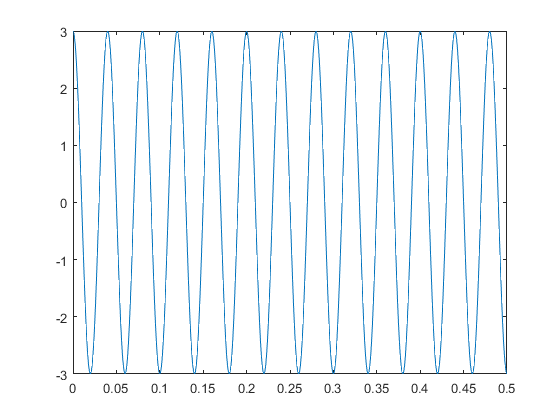
\includegraphics{./pictures/1.png} \\ Рис.1 Сигнал}
\\}

{\itemВыполним фазовую модуляцию, используя функцию pmmod
\center{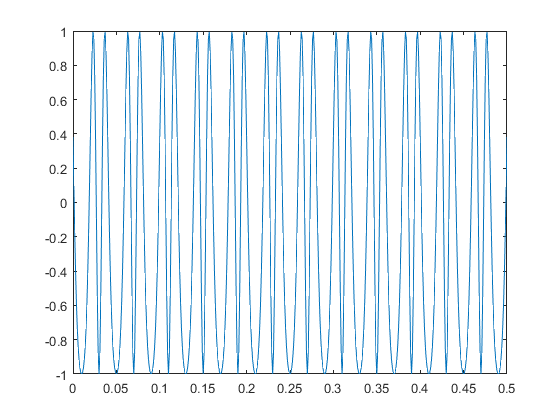
\includegraphics{./pictures/2.png} \\ Рис.2 Амплитудная модуляция}
\center{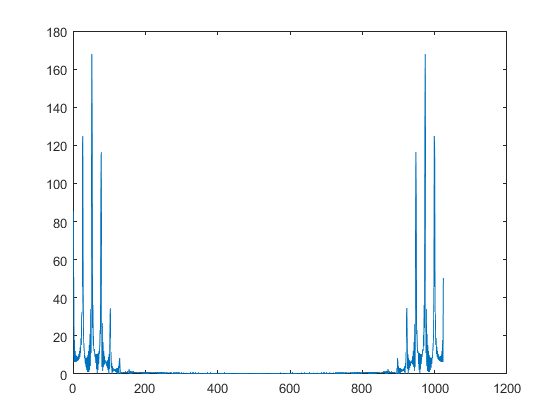
\includegraphics{./pictures/3.png} \\ Рис.3 Спектр сигнала}
\\}

{\itemВыполним демодуляцию ФМ-сигнала.
\center{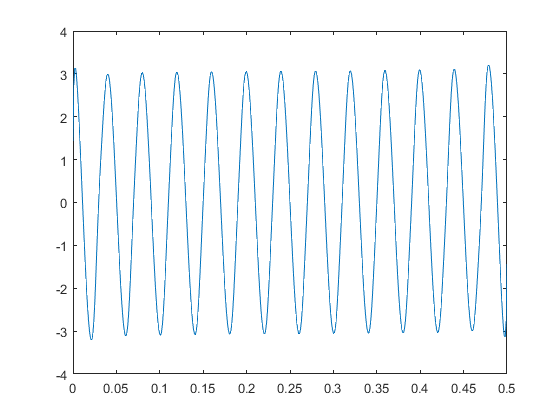
\includegraphics{./pictures/4.png} \\ Рис.4 Модуляция с подавлением несущей}
\center{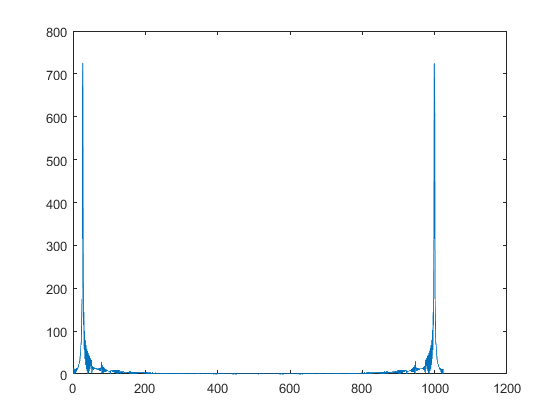
\includegraphics{./pictures/5.png} \\ Рис.5 Спектр сигнала}
\\}

{\itemВыполним частотную модуляцию, используя функцию fmmod.
\center{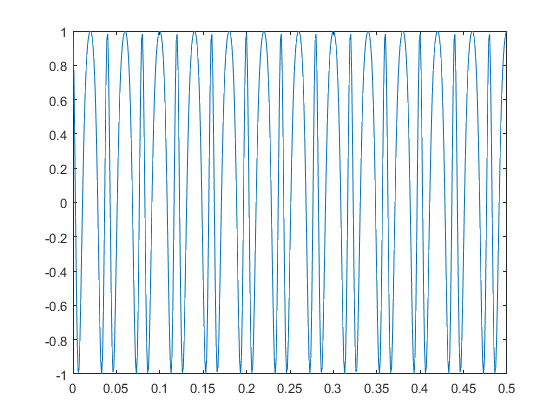
\includegraphics{./pictures/6.png} \\ Рис.6 Однополосная модуляция}
\center{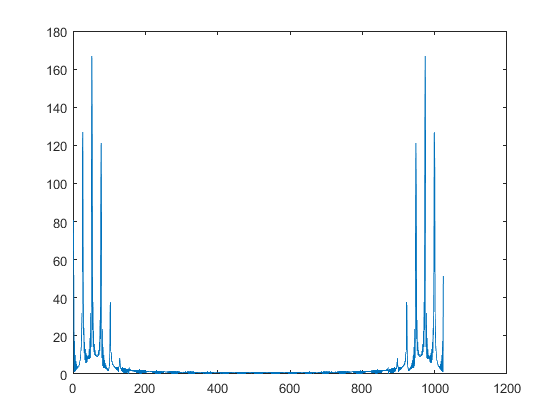
\includegraphics{./pictures/7.png} \\ Рис.7 Спектр сигнала}
\\}

{\itemВыполним демодуляцию ЧМ-сигнала.
\center{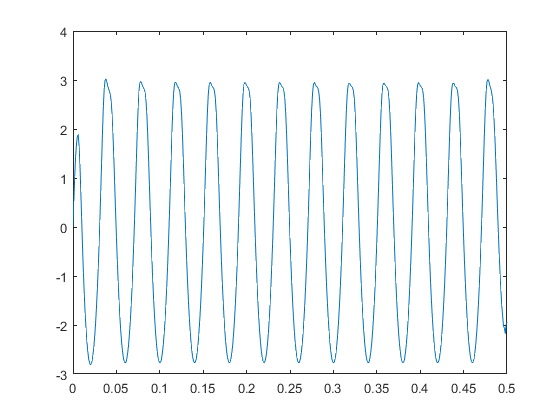
\includegraphics{./pictures/8.png} \\ Рис.8 Сигнал после синхронного детектирования}
\center{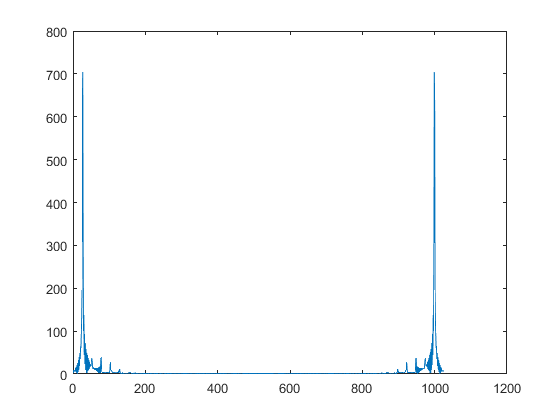
\includegraphics{./pictures/9.png} \\ Рис.9 Спектр сигнала}
\\}

\section{Вывод}

В ходе выполнения лабораторной работы исследована фазовая и частотная модуляция/демодуляция сигналов. Модуляция сигналов находит широкое применение в телекоммуникационных технологиях. Например, используется для высококачественной передачи звукового сигнала в теле- и радиовещании, в сотовой телефонной связи и других системах.

\end{enumerate}
\end{document}
